\chapter{Badania}

 

Rozdział przedstawia przeprowadzone badania. Jest to zasadnicza część i~musi wyraźnie dominować w~pracy.
Badania i analizę wyników należy przeprowadzić, tak jak jest przyjęte w środowisku naukowym (na przykład korzystanie z danych benchmarkowych, walidacja krzyżowa, zapewnienie powtarzalności testów itd). 

\section{Metodyka badań}

\begin{itemize}
\item opis metodyki badań
\item opis stanowiska badawczego (opis interfejsu aplikacji badawczych -- w~załączniku)
\end{itemize}


\section{Zbiory danych}

\begin{itemize}
\item opis danych
\end{itemize}


\section{Wyniki}

\begin{itemize}
\item prezentacja wyników, opracowanie i poszerzona dyskusja  wyników, wnioski
\end{itemize}

 
\begin{table}
\centering
\caption{Opis tabeli nad nią.}
\label{id:tab:wyniki}
\begin{tabular}{rrrrrrrr}
\toprule
	         &                                     \multicolumn{7}{c}{metoda}                                      \\
	         \cmidrule{2-8}
	         &         &         &        \multicolumn{3}{c}{alg. 3}        & \multicolumn{2}{c}{alg. 4, $\gamma = 2$} \\
	         \cmidrule(r){4-6}\cmidrule(r){7-8}
	$\zeta$ &     alg. 1 &   alg. 2 & $\alpha= 1.5$ & $\alpha= 2$ & $\alpha= 3$ &   $\beta = 0.1$  &   $\beta = -0.1$ \\
\midrule
	       0 &  8.3250 & 1.45305 &       7.5791 &    14.8517 &    20.0028 & 1.16396 &                       1.1365 \\
	       5 &  0.6111 & 2.27126 &       6.9952 &    13.8560 &    18.6064 & 1.18659 &                       1.1630 \\
	      10 & 11.6126 & 2.69218 &       6.2520 &    12.5202 &    16.8278 & 1.23180 &                       1.2045 \\
	      15 &  0.5665 & 2.95046 &       5.7753 &    11.4588 &    15.4837 & 1.25131 &                       1.2614 \\
	      20 & 15.8728 & 3.07225 &       5.3071 &    10.3935 &    13.8738 & 1.25307 &                       1.2217 \\
	      25 &  0.9791 & 3.19034 &       5.4575 &     9.9533 &    13.0721 & 1.27104 &                       1.2640 \\
	      30 &  2.0228 & 3.27474 &       5.7461 &     9.7164 &    12.2637 & 1.33404 &                       1.3209 \\
	      35 & 13.4210 & 3.36086 &       6.6735 &    10.0442 &    12.0270 & 1.35385 &                       1.3059 \\
	      40 & 13.2226 & 3.36420 &       7.7248 &    10.4495 &    12.0379 & 1.34919 &                       1.2768 \\
	      45 & 12.8445 & 3.47436 &       8.5539 &    10.8552 &    12.2773 & 1.42303 &                       1.4362 \\
	      50 & 12.9245 & 3.58228 &       9.2702 &    11.2183 &    12.3990 & 1.40922 &                       1.3724 \\
\bottomrule
\end{tabular}
\end{table}  


 
\begin{figure}
\centering
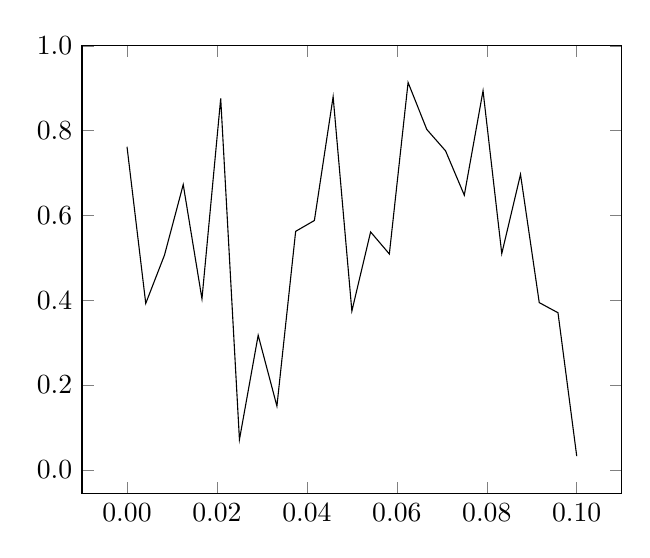
\begin{tikzpicture}
\begin{axis}[
    y tick label style={
        /pgf/number format/.cd,
            fixed,   % po zakomentowaniu os rzednych jest indeksowana wykladniczo
            fixed zerofill, % 1.0 zamiast 1
            precision=1,
        /tikz/.cd
    },
    x tick label style={
        /pgf/number format/.cd,
            fixed,
            fixed zerofill,
            precision=2,
        /tikz/.cd
    }
]
\addplot [domain=0.0:0.1] {rnd};
\end{axis} 
\end{tikzpicture}
\caption{Podpis rysunku po rysunkiem.}
\label{fig:2}
\end{figure}


\begin{figure}
\begin{lstlisting}
if (_nClusters < 1)
	throw std::string ("unknown number of clusters");
if (_nIterations < 1 and _epsilon < 0)
	throw std::string ("You should set a maximal number of iteration or minimal difference -- epsilon.");
if (_nIterations > 0 and _epsilon > 0)
	throw std::string ("Both number of iterations and minimal epsilon set -- you should set either number of iterations or minimal epsilon.");
\end{lstlisting}
\caption{Przykład pseudokodu}
\end{figure}


\section{Metodyka badań}

\begin{figure}
\centering
\begin{subfigure}{0.8\textwidth}
    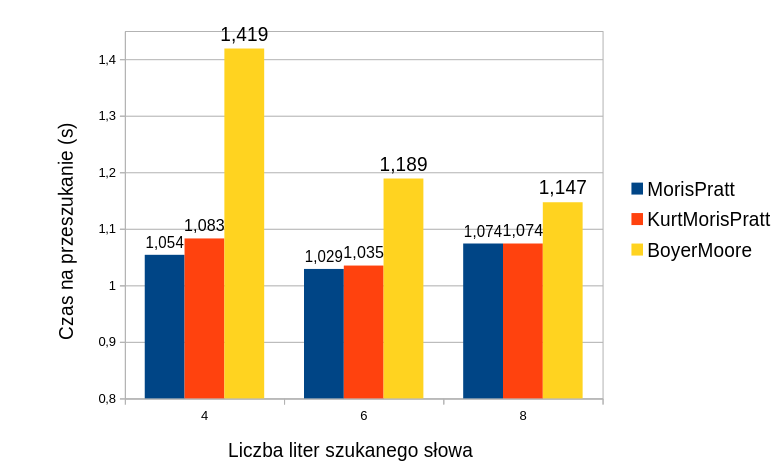
\includegraphics[width=\textwidth]{./images/GraphFirstAttempt.png}
    \caption{Wykres czasów bez statycznego bufora oraz z ponownym rekalkujacją
    bufora pre alokowanego.}
    \label{fig:GraphFirstAttempt}
\end{subfigure}
%\hfill
\begin{subfigure}{0.8\textwidth}
    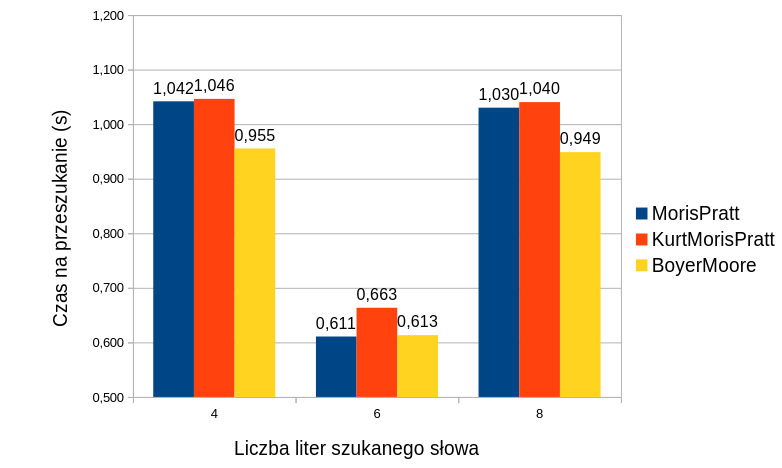
\includegraphics[width=\textwidth]{./images/GraphPreAllocBM.png}
    \caption{Wykres czasów bez statycznego bufora z kalkulacją bufora 
    prealokowanego dla algorytmu Boyer Moore'a. }
    \label{fig:GraphPreAllocBM}
\end{subfigure}
\begin{subfigure}{0.8\textwidth}
%TODO dodac grafike
    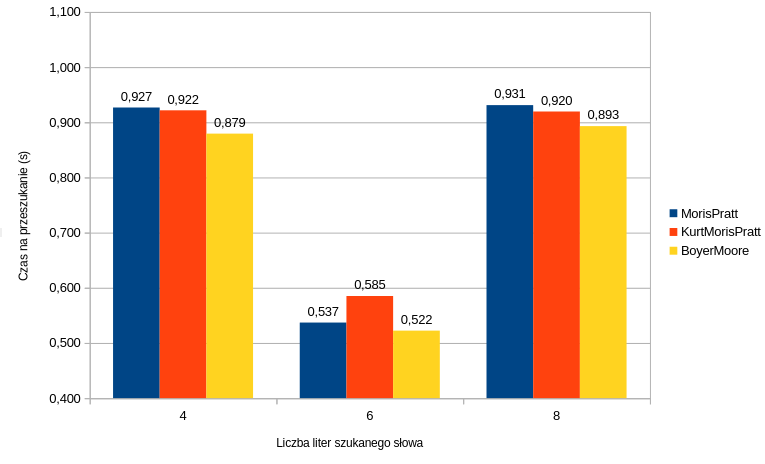
\includegraphics[width=\textwidth]{./images/GraphStaticPreallocAndFileBuffer.png}
    \caption{Wykres czasów z statycznym buforem prealokacji oraz statycznym buforem
    dla zawartości pliku.}
    \label{fig:GraphStaticPreallocAndFileBuffer}
\end{subfigure}
\caption{Wykresy kolejnych iteracji na algorytmach}
\label{fig:GraphsIterationComparison}
\end{figure}
%Rys. \ref{fig:GraphsIterationComparison} przestawia wiele ważnych informacji, np. rys. \ref{fig:prawy-gorny} jest na prawo u góry.

Pierwszy test wydajnościowy, który został przeprowadzony, sprawdzał wszystkie 
foldery, w których znajdowały się pliki, które nie miałyby sensu by być odczytane
przez algorytm. Wykonano testy na 3 algorytmach, gdzie odczytywano 5191 plików 
i łącznie 240 MB danych. Oto rezultaty określonych algorytmów.

Algorytm Morisa-Pratta jest nieznacznie wolniejszy od algorytmu 
Kurta-Morisa-Pratta. Jest to spowodowane niewielką optymalizacją pomiędzy tymi 
dwoma algorytmami. Według danych na rysunku \ref{fig:GraphFirstAttempt} można 
zauważyć, KMP w niektórych przypadkach jest wolniejszy, niż algorytm MP, 
ponieważ posiada większe odchylenie standardowe, co powoduje, że jest mniej
stabilny. 

Patrząc na statystki możemy zauważyć, że podczas pracy algorytmów, wystąpiły 
wartości odstające (ang. \english{Outlier}) w niektórych wykonaniach dla 
algorytmu KMP. Gdy usuniemy je pojawia się bardziej rzetelna informacja o 
różnicy pomiędzy wynikami
%TODO start here, make use of python
%
%[gadzbi@fedora baza_mgr_large]$ python3 mime_stats.py
%application/pdf                               1094989.16 KB      656
%application/zip                                911563.68 KB      153
%application/x-rar                              751425.98 KB       34
%application/gzip                               158709.61 KB      126
%application/postscript                         151226.98 KB      488
%text/html                                       49879.89 KB     2473
%image/jpeg                                      49342.96 KB     5303
%image/gif                                       42260.80 KB     2353
%text/xml                                        16914.17 KB     1233
%application/x-tar                               10470.00 KB        9
%application/mac-binhex40                         4704.44 KB        2
%text/plain                                       2929.91 KB      285
%application/octet-stream                         2131.61 KB       56
%application/vnd.microsoft.portable-executable    1552.50 KB        2
%application/x-ms-ne-executable                   1404.35 KB        1
%text/x-c++                                       1139.31 KB      121
%application/x-ace-compressed                     1004.49 KB        1
%application/msword                                460.50 KB        3
%application/x-compress-ttcomp                     362.78 KB        2
%text/x-c                                          332.51 KB      134
%application/x-java-applet                         293.44 KB      270
%application/x-msaccess                            154.00 KB        1
%application/x-dosexec                             117.99 KB        3
%text/x-java                                        94.38 KB       49
%application/vnd.ms-cab-compressed                  88.34 KB        2
%text/csv                                           54.14 KB       64
%text/x-diff                                        46.94 KB        2
%application/vnd.openxmlformats-officedocument.wordprocessingml.document      34.65 KB        2
%text/x-script.python                                1.90 KB        1
%inode/x-empty                                       0.00 KB        2
%Total                                         3253691.41 KB    13831


TODO DIFF IMPLEMENTACJI

Algorytm Boyera-Moore'a wykorzystywany w takich narzędziach jak Grep, posiada
wolniejszy czas egzekucji, ale algorytm może zostać napisany w lepszy sposób, 
aby otrzymać lepszy rezultat.

TODO SLOW BOYER
PORÓWNANIE STATYSTYK ALGOS

Następna implementacja korzysta z algorytmu ze strony na githubie 
\cite{bib:internet:BoyerMooreGit}. Jest ona znacznie wolniejsza od pozostałych
algorytmów, dlatego że znaczną cześć czasu spędzamy na stworzeniu tablicy
pre-procesora. Jako że zawsze sprawdzamy ten sam ciąg w wszystkich plikach w
folderze, możemy stworzyć tablice pre-procasora przy pierwszym użyciu algorytmu,
a następnie wykorzystywanie tej tablicy w wszystkich odczytach. To spowodowało, 
że czasy wykonania algorytmu boyer moora są znacznie szybsze od pozostałych.

PORÓWNANIE STATYSTYK ALGOS

Dodatkową poprawą egzekucji algorytmów było ponowne wykorzystanie bufora, do 
którego odczytywane zawartości plików. Powoduje to niestety, że należy wiedzieć
jaki będzie rozmiar największego pliku, który odczytamy (11 MB bez plików 
archiwów). Moglibyśmy przed rozpoczęciem algorytmu sprawdzać rozmiar maksymalny 
pliku ale to wydłuży czas działania. Istnieje też sytuacja w której nie 
chcielibyśmy tego ograniczać. 

PORÓWNANIE PAMIECI ALGOS

